\subsection{Risultati sperimentali}
Proponiamo alcuni risultati sperimentali ottenuti dal package Python contenente gli algoritmi per il calcolo della bisimulazione massima che abbiamo presentato nelle sezioni precedenti. Innanzitutto illustreremo brevemente l'ambiente e gli strumenti con cui sono state prese le misurazioni. Dopodichè presenteremo i risultati in forma di grafici, e tenteremo di evidenziare le differenze tra i vari algoritmi.

\subsubsection{Hardware e strumenti per le misura}
I risultati sono stati misurati su un computer con sistema operativo \emph{CentOS Linux}, architettura x86\_64, processore \emph{Intel(R) Core(TM) i7-4790 CPU} (4 cores, 3.60GHz), e memoria RAM da 16 GB. Per ottenere le misurazioni è stato utilizzato il package Python \emph{timeit}, che presenta alcune caratteristiche che lo rendono un valido strumento per la misurazione del tempo di esecuzione \cite{pythondocs}:
\begin{itemize}
    \item Utilizza la più precisa funzione disponibile sulla piattaforma per la misurazione del tempo trascorso;
    \item Disabilita il \emph{garbage collector}, che potrebbe intervenire in un momento casuale della misurazione introducendo rumore nei risultati;
    \item Esegue lo script preso in esame molte volte (il numero è deciso dall'utilizzatore) in modo da ridurre il rumore dovuto a temporanei sovraccarichi della CPU o della RAM.
\end{itemize}

I dataset su cui abbiamo effettuato le misurazioni sono stati generati utilizzando alcune funzioni del package Python \emph{NetworkX} \cite{networkx}.

\subsubsection{Performance}
Consideriamo alcune tipologie differenti di grafi, e valutiamo il tempo di esecuzione necessario per l'esecuzione degli algoritmi che abbiamo implementato. Nei grafici abbiamo rimpiazzato ad ogni grafo il corrispondente valore di $|V| \log |E|$, ed abbiamo utilizzato questa scala per l'asse delle ascisse, in quanto è lecito supporre che questo ci consenta di avere un andamento abbastanza lineare per gli algoritmi implementati.

Cominciamo l'esposizione dei risultati con la categoria dei grafi chiamati ``alberi bilanciati'', ovvero grafi che possono essere rappresentati nella forma esposta nella Figura \ref{fig:balanced_tree}. Essi sono caratterizzati da due parametri:
\begin{itemize}
    \item \emph{depth}: determina il numero di livelli (senza contare la \emph{root});
    \item \emph{branching factor}: il numero di successori di ogni nodo, ad eccezione dei nodi dell'ultimo livello.
\end{itemize}
Generiamo grafi di questo tipo tramite la funzione \verb|balanced_tree| di \emph{NetworkX}, che appunto prende in input questi due parametri.

\begin{figure}
    \centering
    \begin{subfigure}[b]{0.4\textwidth}
        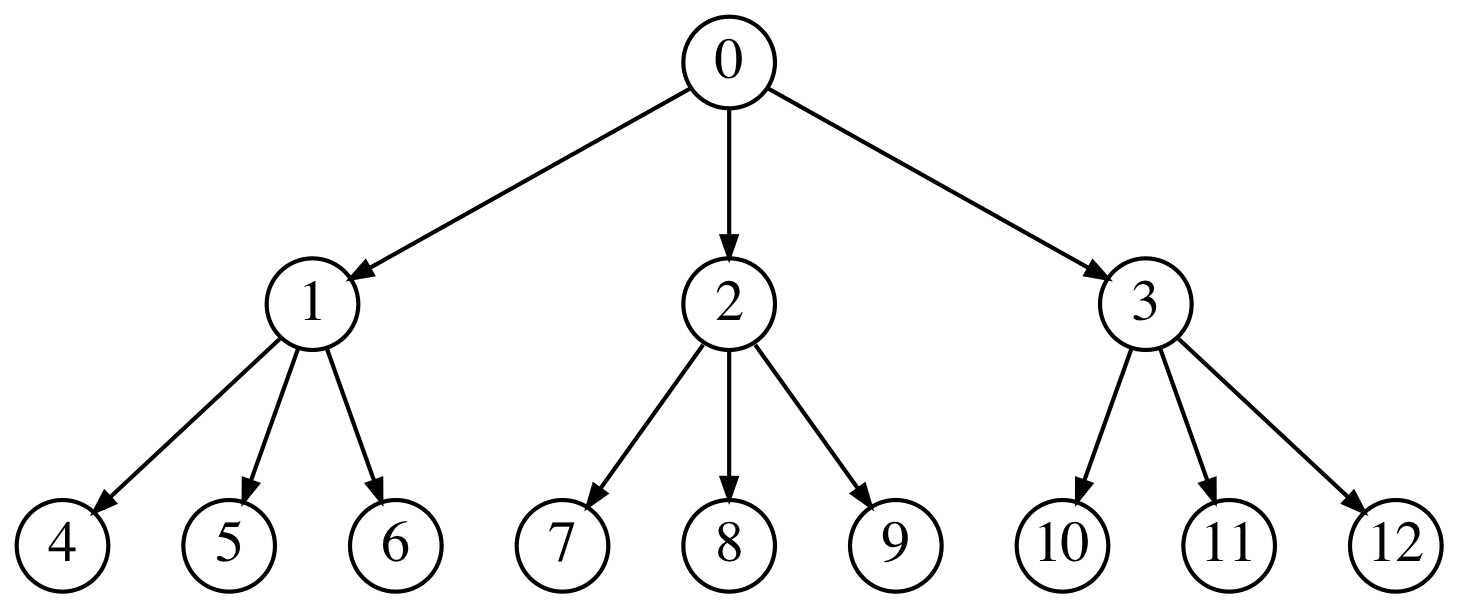
\includegraphics[width=\textwidth]{./sezione3/experimental_results/plots/tree_graph.png}
        \caption{Un albero bilanciato, \emph{depth}=2, \emph{branching factor}=3.}
        \label{fig:balanced_tree}
    \end{subfigure}
    \qquad
    \begin{subfigure}[b]{0.1\textwidth}
        \centering
        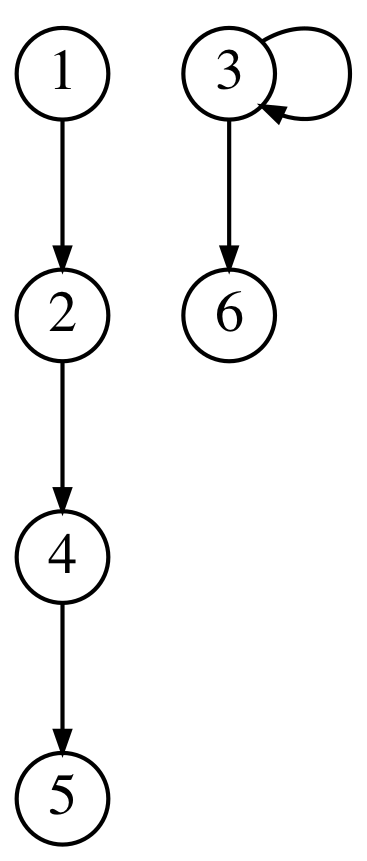
\includegraphics[width=\textwidth]{./sezione3/experimental_results/plots/hopcroft_graph_1.png}
        \caption{Hopcroft, $n=2$}
        \label{fig:hopcroft_graph_1}
    \end{subfigure}
    \qquad \qquad
    \begin{subfigure}[b]{0.2\textwidth}
        \centering
        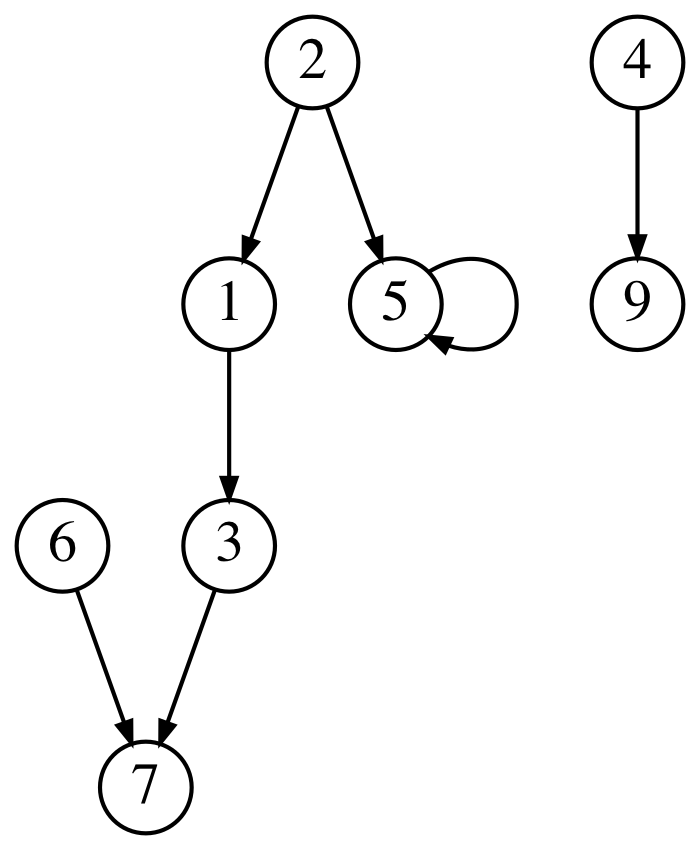
\includegraphics[width=\textwidth]{./sezione3/experimental_results/plots/hopcroft_graph_2.png}
        \caption{Hopcroft, $n=3$}
        \label{fig:hopcroft_graph_2}
    \end{subfigure}
    \caption{Tipologie di grafi su cui abbiamo testato gli algoritmi di Dovier-Piazza-Policriti e Paige-Tarjan.}
\end{figure}

Dalla Figura \ref{fig:tree_exp_result} possiamo osservare che asintoticamente l'algoritmo di Dovier-Piazza-Policriti è asintoticamente più efficiente, a partire da un certo valore di $|E| \log |V|$. Sebbene intuitivamente la metodologia sia più ``rifinita'' dell'approccio di Paige-Tarjan, lo sforzo iniziale per il calcolo del rango è non indifferente, soprattutto se consideriamo il linguaggio in cui l'algoritmo è stato implementato. Abbiamo però la conferma che per valori alti di $|E| \log |V|$, per questa tipologia di grafo, si ottengono i risultati previsti.

\begin{figure}
    \makebox[\linewidth][c]{
        \begin{subfigure}[b]{0.6\textwidth}
            \centering
            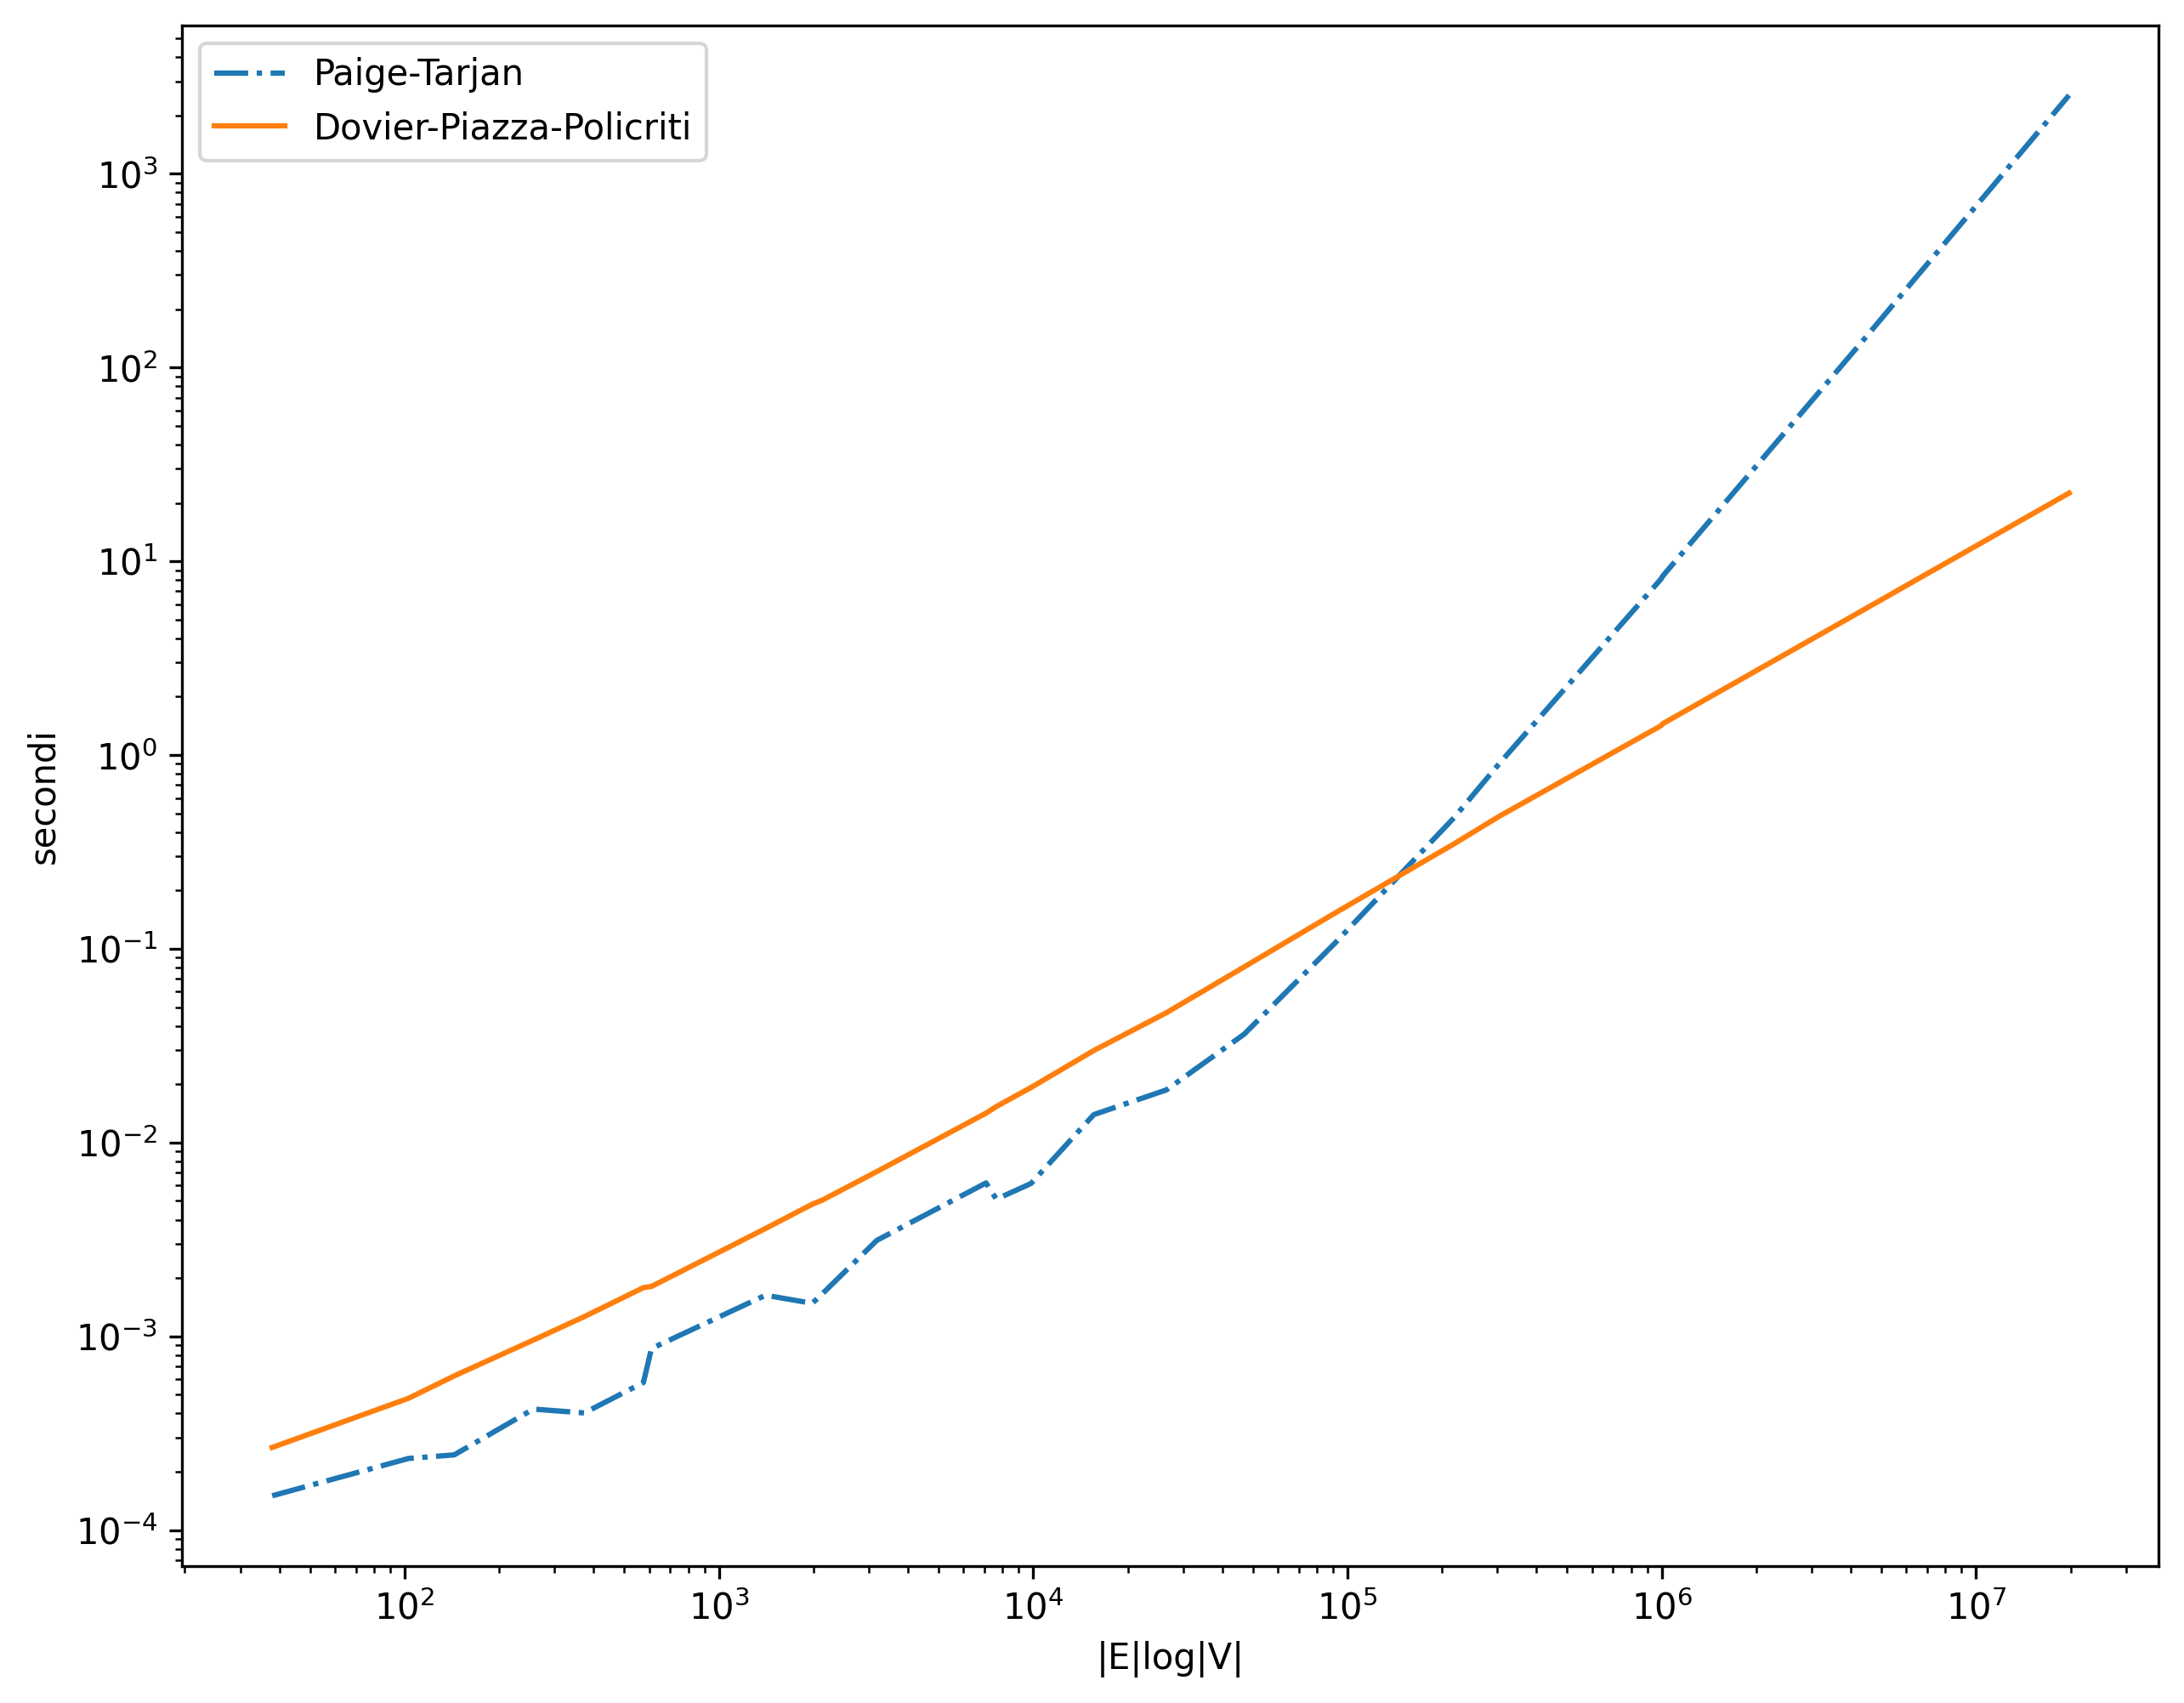
\includegraphics[width=0.7\textwidth]{./sezione3/experimental_results/plots/tree.png}
            \caption{Performance su alberi bilanciati con \emph{depth} e \emph{branching factor} variabili.}
            \label{fig:tree_exp_result}
        \end{subfigure}
        \qquad
        \begin{subfigure}[b]{0.6\textwidth}
            \centering
            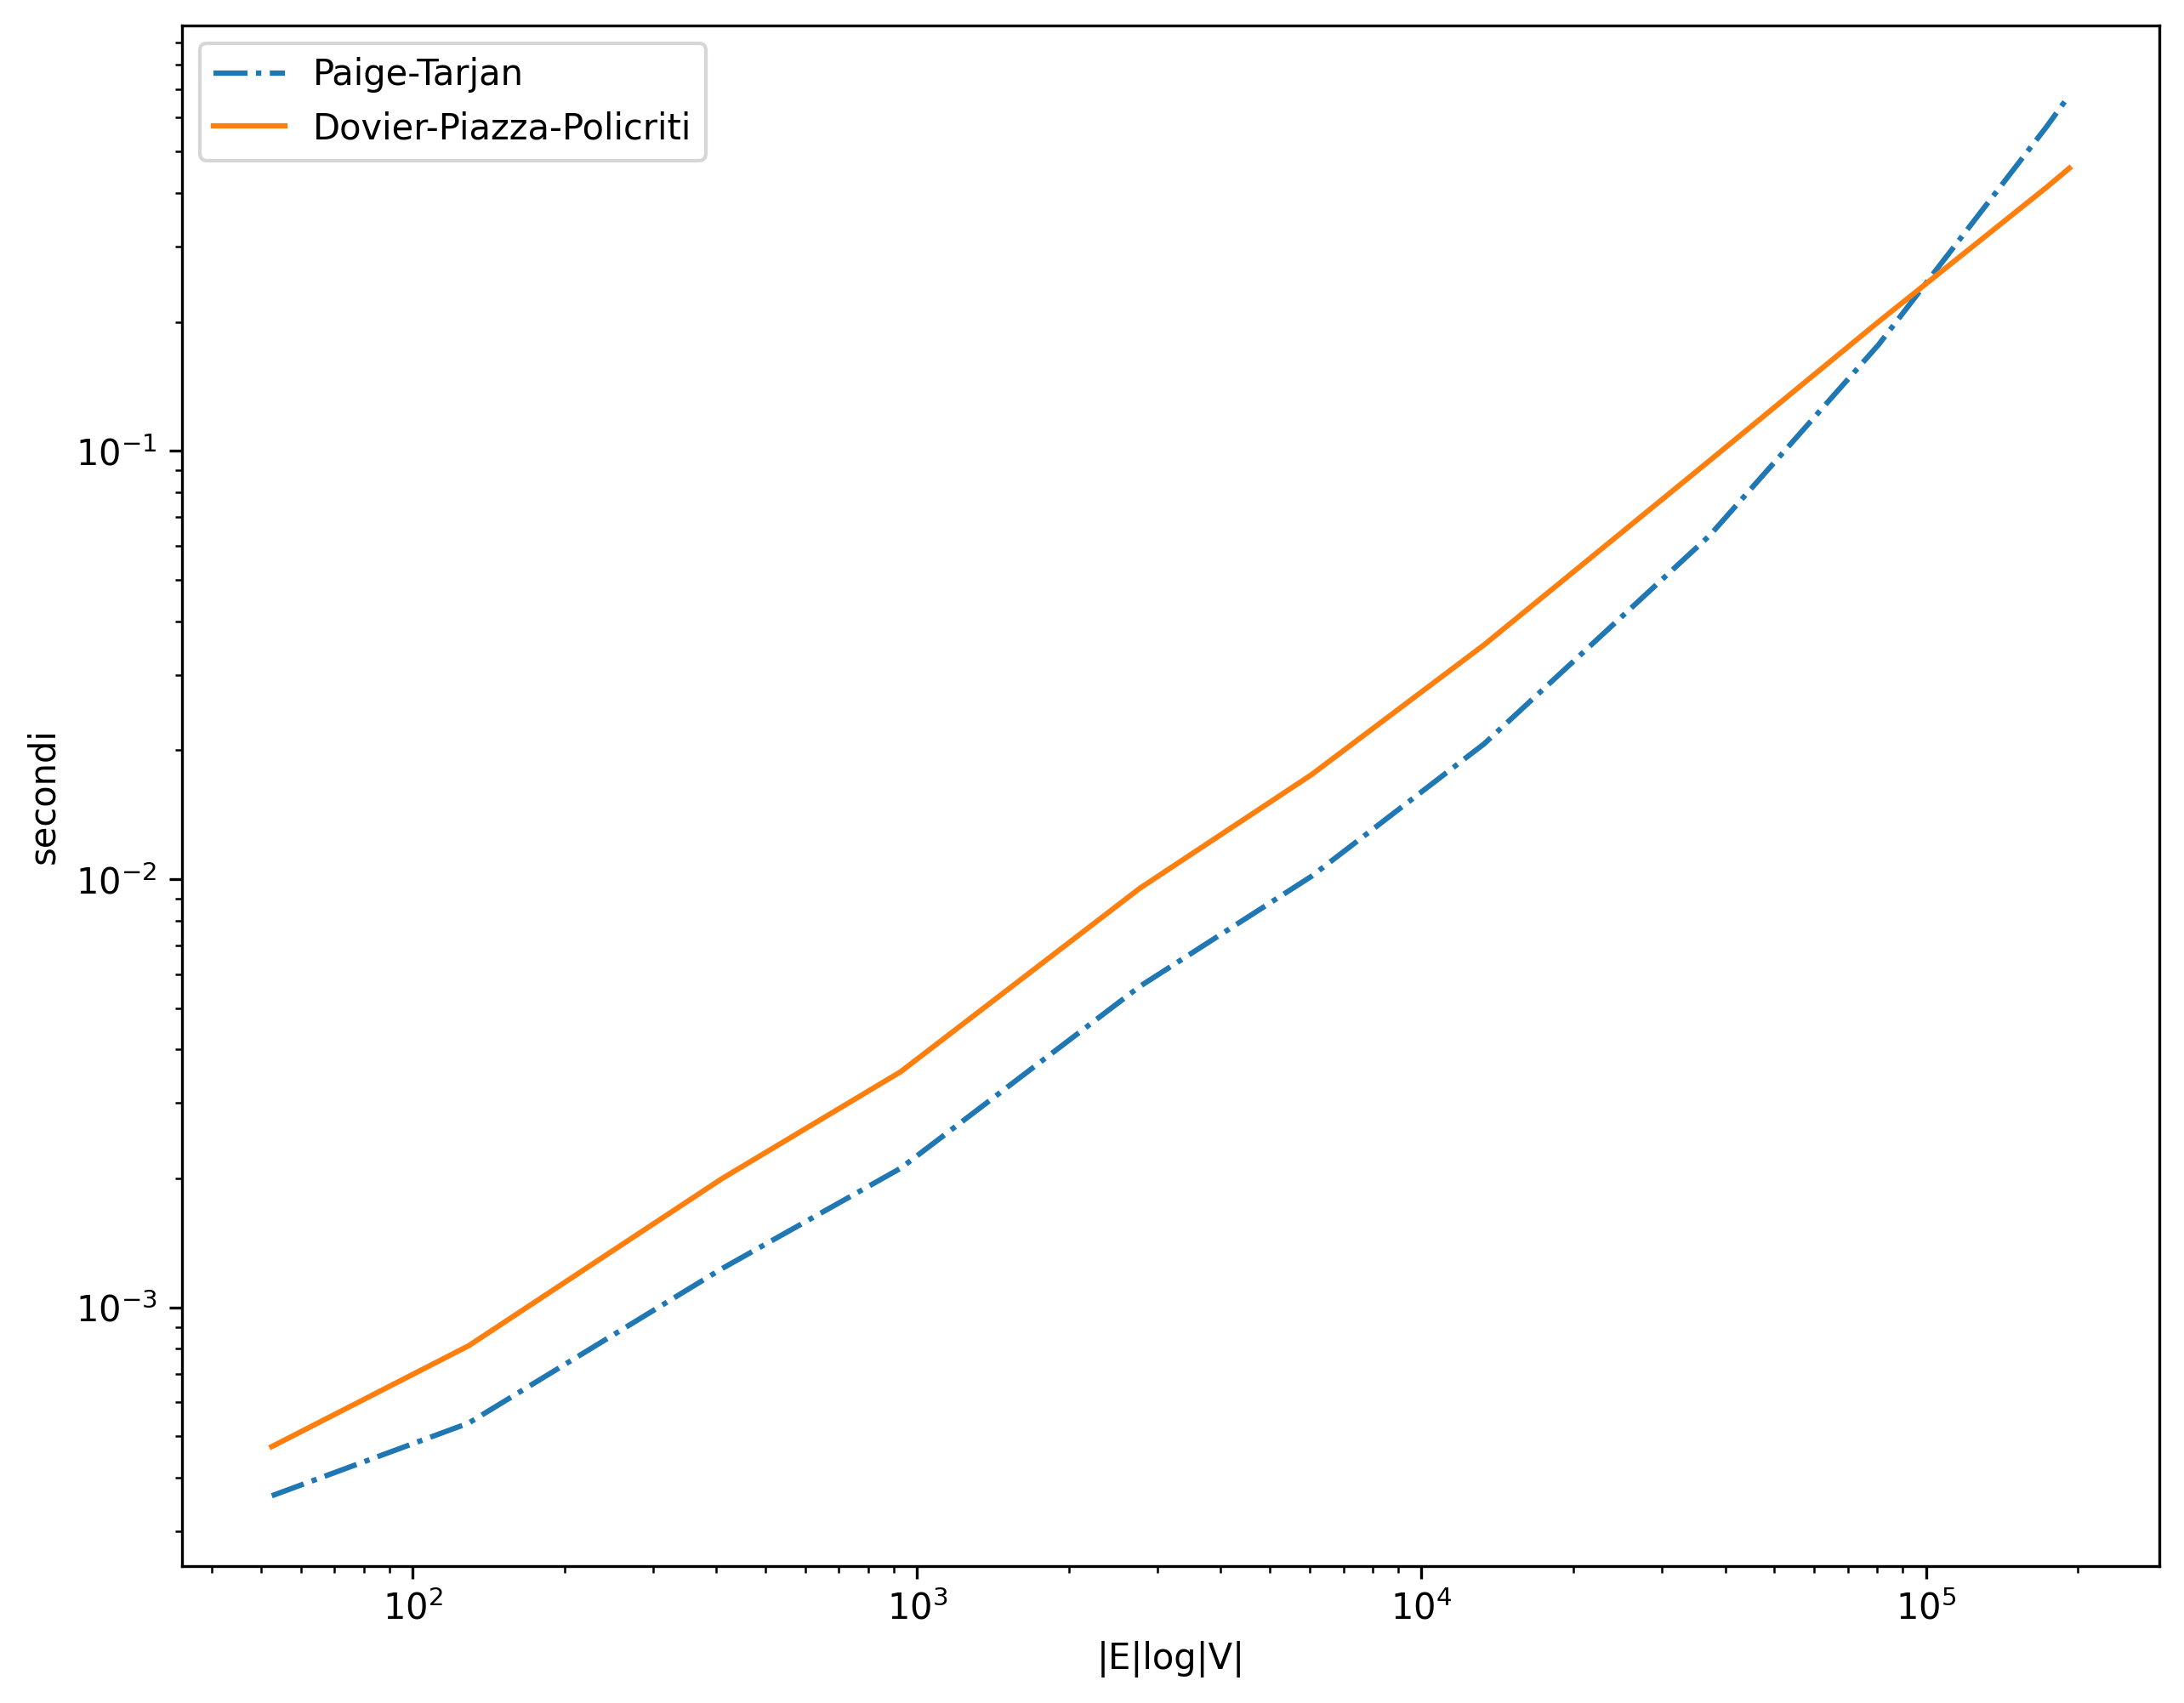
\includegraphics[width=0.7\textwidth]{./sezione3/experimental_results/plots/hopcroft.png}
            \caption{Performance su grafi della tipologia proposta da Hopcroft di dimensioni varie.}
            \label{fig:hopcroft_exp_result}
        \end{subfigure}
    }
    \caption{Tempo di esecuzione degli algoritmi di Dovier-Piazza-Policriti e Paige-Tarjan sulle tipologie di grafi testate.}
\end{figure}

La seconda tiplogia di grafi che consideriamo è tratta dal paper in cui viene presentato l'algoritmo di Dovier-Piazza-Policriti, ed è un esempio di automa proposto originariamente da Hopcroft \cite{hopcroft}. Nelle Figure \ref{fig:hopcroft_graph_1} e \ref{fig:hopcroft_graph_2} visualizziamo alcune realizzazioni di questa tipologia di grafo.

In Figura \ref{fig:hopcroft_exp_result} sono riportati i risultati ottenuti dagli algoritmi di Paige-Tarjan e Dovier-Piazza-Policriti, mantenendo la quantità $|E| \log |V|$ nell'asse delle ascisse. Come prima, possiamo osservare un andamento abbastanza lineare dei due algoritmi nella scala che abbiamo adottato, e vediamo che l'algoritmo di Dovier-Piazza-Policriti risulta asintoticamente più conveniente anche in questo caso.

\subsubsection{Dimensione della bisimulazione massima}
Terminiamo la sezione relativa ai risultati sperimentali con un'ultima analisi che potrebbe essere di qualche interesse nella prospettiva di ciò che abbiamo presentato nella Sezione \ref{sec:applitations}. Consideriamo l'andamento del numero di classi di equivalenza nella bisimulazione massima per grafi di Erdős-Rényi (o \emph{grafi binomiali}), ovvero grafi contenenti un numero arbitrario \verb|n| di nodi, per cui presa una coppia qualsiasi $u,v \in V$ si ha $\langle u,v\rangle \in E$ con probabilità \verb|p| $< 1$.
Considereremo valori piccoli di \verb|p|, in quanto avvicinandoci ad 1 otteniamo grafi sempre più ``completi'' di interesse molto basso nella pratica.

\begin{figure}
    \makebox[\textwidth][c]{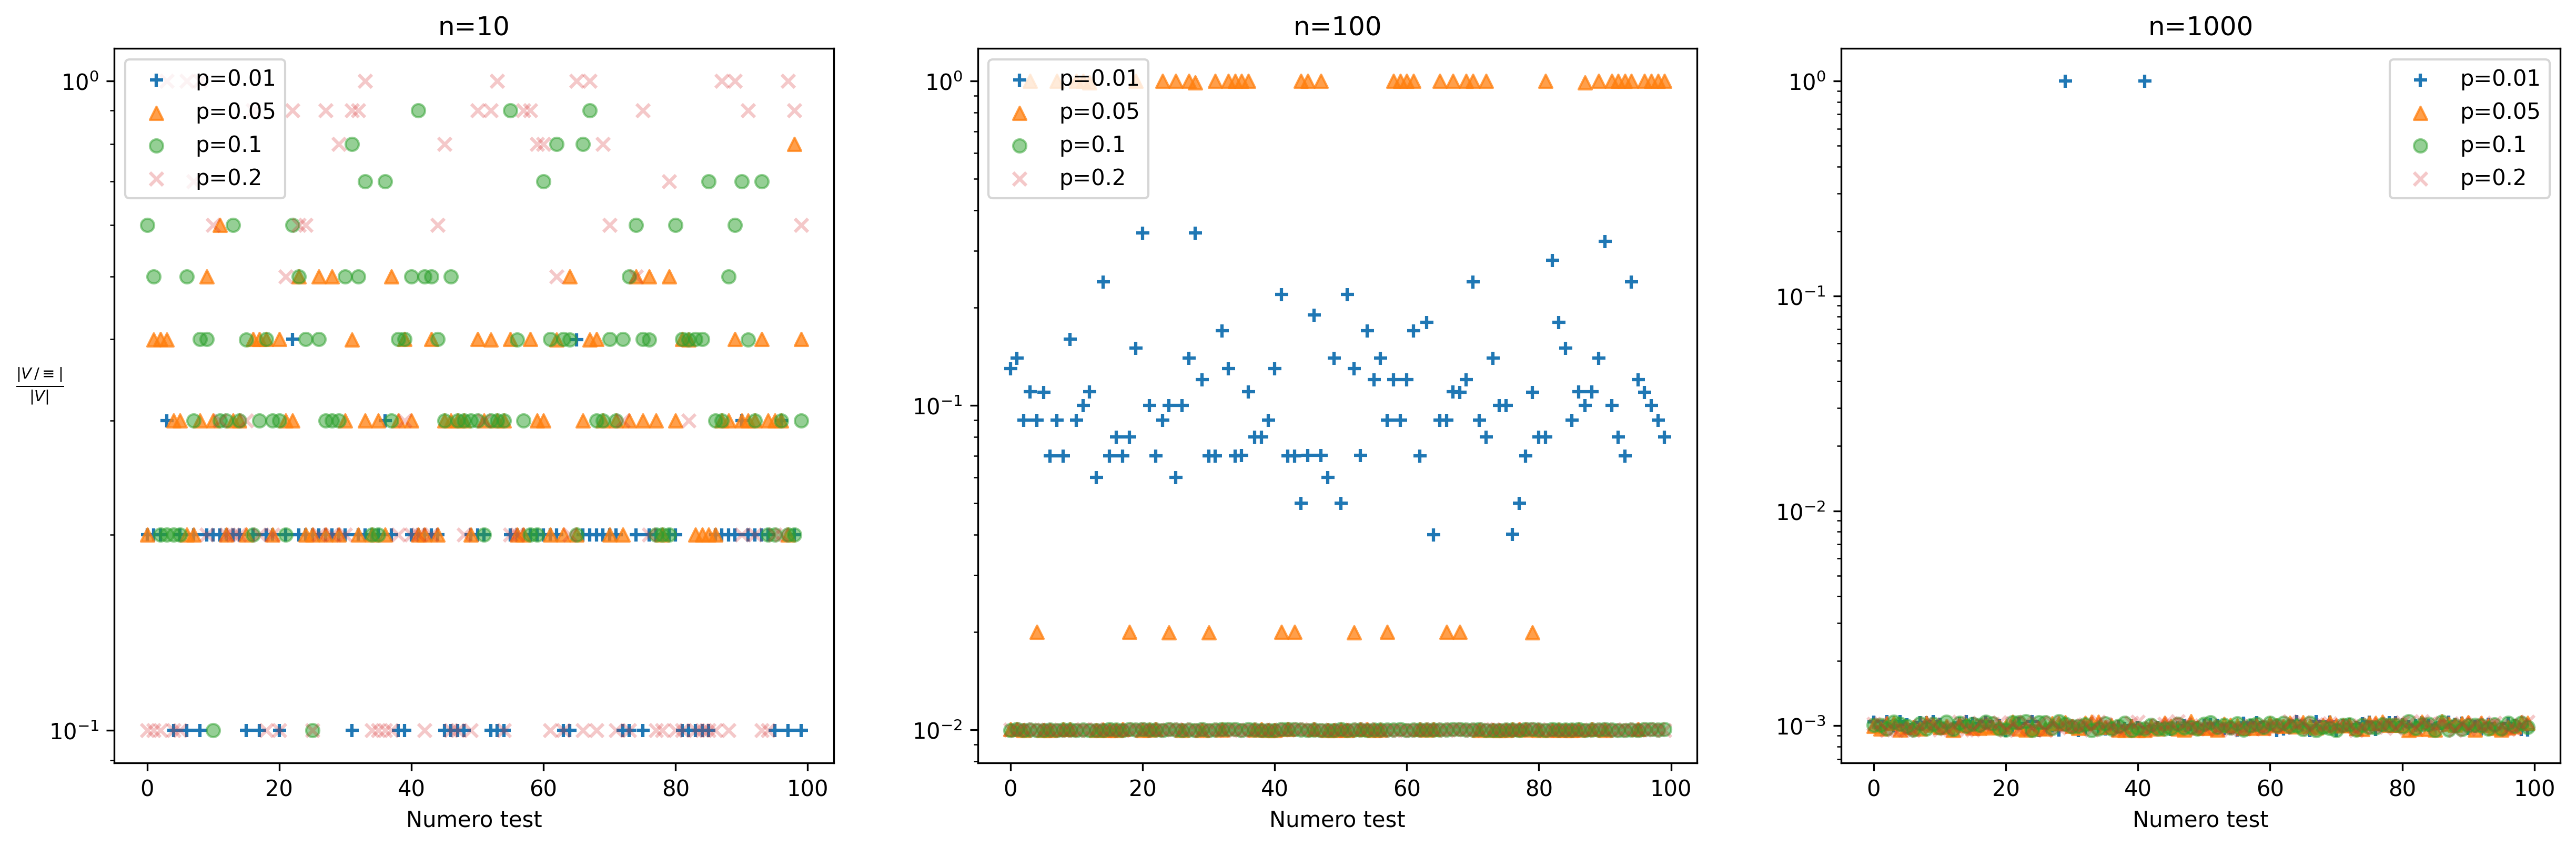
\includegraphics[width=1.2\textwidth]{./sezione3/experimental_results/plots/bisize.png}}
    \caption{Numero di classi di equivalenza della bisimulazione massima per grafi generati in modo casuale, normalizzato con il numero di nodi nel grafo.}
    \label{fig:bisi_size}
\end{figure}

Nella Figura \ref{fig:bisi_size} abbiamo tre diversi valori di \verb|n|, ed in ogni sotto-immagine abbiamo considerato i valori 0.01, 0.05, 0.1, 0.2 per \verb|p|. Per ogni combinazione di \verb|n|,\verb|p| abbiamo generato 100 grafi binomiali con la funzione \verb|fast_gnp_random_graph| del pacchetto \emph{NetworkX}, e ne abbiamo valutata la bisimulazione massima con l'algoritmo di \emph{Dovier-Piazza-Policriti}. Nei grafici abbiamo visualizzato la quantità $\frac{|V / \equiv|}{|V|}$, ovvero il rapporto tra il numero di classi di equivalenza nella bisimulazione massima ed il numero di nodi del grafo: questa quantità potrebbe essere considerata come il fattore di riduzione che otteniamo quanto sostuitiamo al grafo originale la sua contrazione secondo la bisimulazione massima.

Possiamo vedere in modo abbastanza evidente che per \verb|n=10| la quantità che stiamo valutando varia molto tra 1 (10 classi di equivalenza, nessuna riduzione) e 0.1 (tutti i nodi sono bisimili, riduzione massima). Per valori più grandi questa variabilità si riduce, e per \verb|n=1000| il fattore si schiaccia decisamente verso 0.001 (un'unica partizione).

Se la riduzione può essere un risultato positivo, bisogna anche considerare che gran parte dell'informazione veicolata dal grafo originale viene persa. Infatti, se da 1000 nodi passiamo ad un solo nodo non vi può essere che un unico arco. A seconda delle applicazioni questa contrazione potrebbe risultare interessante o scoraggiante; si potrebbe tentare di correggere il risultato assegnando delle etichette ai nodi per imporre un partizionamento preventivo, che dovrà essere rispettato anche dalla bisimulazione massima.

Si ricordi comunque che questo è un caso molto particolare, in quanto appunto generiamo il grafo in modo del tutto casuale. Nelle applicazioni pratiche solitamente è facile individuare una struttura fondamentale: ad esempio, se intendiamo modellizzare un social network, è probabile che si possano individuare ``cluster'' di nodi relativi ad account i cui proprietari vivono geograficamente vicini.
